% !TEX TS-program = pdflatex
% !TEX encoding = UTF-8 Unicode

% This is a simple template for a LaTeX document using the "article" class.
% See "book", "report", "letter" for other types of document.

\documentclass[twocolumn]{article} % use larger type; default would be 10pt

\usepackage[utf8]{inputenc} % set input encoding (not needed with XeLaTeX)

%%% Examples of Article customizations
% These packages are optional, depending whether you want the features they provide.
% See the LaTeX Companion or other references for full information.

%%% PAGE DIMENSIONS
\usepackage[twocolumn, columnsep=.2in]{geometry} % to change the page dimensions
\geometry{letterpaper} % or letterpaper (US) or a5paper or....
\geometry{margin=.75in} % for example, change the margins to 2 inches all round
% \geometry{landscape} % set up the page for landscape
%   read geometry.pdf for detailed page layout information
\usepackage{multirow}

\usepackage{graphicx} % support the \includegraphics command and options

% \usepackage[parfill]{parskip} % Activate to begin paragraphs with an empty line rather than an indent

%%% PACKAGES
\usepackage{booktabs} % for much better looking tables
\usepackage{array} % for better arrays (eg matrices) in maths
\usepackage{paralist} % very flexible & customisable lists (eg. enumerate/itemize, etc.)
\usepackage{verbatim} % adds environment for commenting out blocks of text & for better verbatim
\usepackage{subfig} % make it possible to include more than one captioned figure/table in a single float
\usepackage{multicol}
\usepackage{mathtools}
\usepackage{algorithmicx}
\usepackage{algpseudocode}
\usepackage{tikz}
\usepackage{todonotes}
% These packages are all incorporated in the memoir class to one degree or another...

\usepackage{hyperref}
\hypersetup{
    bookmarks=true,         % show bookmarks bar?
    unicode=false,          % non-Latin characters in Acrobat’s bookmarks
    pdftoolbar=true,        % show Acrobat’s toolbar?
    pdfmenubar=true,        % show Acrobat’s menu?
    pdffitwindow=false,     % window fit to page when opened
    pdfstartview={FitH},    % fits the width of the page to the window
    pdftitle={Parallelization Issues},    % title
    pdfauthor={Olav Emil Eiksund},     % author
    pdfsubject={A survey of issues faced when parallelizing algorithms},   % subject of the document
    pdfcreator={Olav Emil Eiksund},   % creator of the document
    pdfproducer={Producer}, % producer of the document
    pdfkeywords={Parallelization} {Particle-In-Cell} {AI}, % list of keywords
    pdfnewwindow=true,      % links in new PDF window
    colorlinks=true,       % false: boxed links; true: colored links
    linkcolor=red,          % color of internal links (change box color with linkbordercolor)
    citecolor=red,        % color of links to bibliography
    filecolor=magenta,      % color of file links
    urlcolor=blue           % color of external links
}

%%% HEADERS & FOOTERS
%\usepackage{fancyhdr} % This should be set AFTER setting up the page geometry
%\pagestyle{fancy} % options: empty , plain , fancy
%\renewcommand{\headrulewidth}{0pt} % customise the layout...
%\lhead{}\chead{}\rhead{}
%\lfoot{}\cfoot{\thepage}\rfoot{}

%%% SECTION TITLE APPEARANCE
\usepackage{sectsty}
\allsectionsfont{\sffamily\mdseries\upshape} % (See the fntguide.pdf for font help)
% (This matches ConTeXt defaults)

%%% ToC (table of contents) APPEARANCE
\usepackage[nottoc,notlof,notlot]{tocbibind} % Put the bibliography in the ToC
\usepackage[titles,subfigure]{tocloft} % Alter the style of the Table of Contents
\renewcommand{\cftsecfont}{\rmfamily\mdseries\upshape}
\renewcommand{\cftsecpagefont}{\rmfamily\mdseries\upshape} % No bold!

%%% END Article customizations

%%% The "real" document content comes below...

\title{Parallelization Issues}
\author{Olav Emil Eiksund, NTNU}
\date{} % Activate to display a given date or no date (if empty),
         % otherwise the current date is printed 

\begin{document}
\twocolumn[\maketitle]

%% Abstract %%
\abstract{
	In this paper a number of parallelization approaches have been examined, with a focus on issues encountered, and how
	they are resolved or bypassed. The selection is from the fields of numerics, data management, and AI, and represent
	quite different problems.
	}

%% Particle-In-Cell codes %%
\section*{Parallelization Issues and Particle-In-Cell Codes}
	\subsection*{Problem}
		Particle simulations attempt to model the behavior and interactions of particles and their forces, with applications
		in for example fluid dynamics or studies of plasma, they tend to be very compute intensive. One type of simulations is
		called Particle-in-cell codes.
		
		Particle-in-cell simulations consist of finding the electrical charge distribution resulting from the particle charges,
		solving the field to find the electrical potential, and move the particles based on the resulting electrical force and
		their current velocity. The simulation is discrete in both time and space and sufficient resolution in either is
		necessary to avoid aliasing, and properly model physical phenomena such as plasma wave oscillation.
	
	\subsection*{Algorithm}
		Pseudocode for the algorithm used by \cite{elster94} is given below, with implementation details abstracted away. \\
		\begin{figure}[h]
		\begin{algorithmic}
			\While{$SimulationIsRunning()$}
				\ForAll{$p \text{ in } particles$}
					\State $chargeDistr[p.position] \text{ += } p.charge$
				\EndFor
				\State $potential = Solve(chargeDistribution)$
				\State
				\Comment{$\text{Solve using ex. FFT or SOR.}$}
				\ForAll{$point \text{ in } grid$}
					\State $elField[point] = -Div(potential[point])$
				\EndFor
				\ForAll{$p \text{ in } particles$}
					\State $elF = ElectricalForce(elField, p.position)$
					\State $p = UpdateVelocity(elF, p.velocity)$
					\State $p = UpdatePosition(p.velocity, p.position)$
				\EndFor
			\EndWhile
		\end{algorithmic}
		\end{figure}
		
		It is apparent from the algorithm that all steps has potential for parallelization. Some important features are
		abstracted away however, such as the grid being discrete. This can lead to write conflicts as particle positions are
		interpolated on the grid.
		
		Also simplified is the solver step, which will be computationally heavy. The two solvers mentioned by \cite{elster94} are the 2D
		Fast Fourier Transform (2D-FFT) and Successive Over Relaxation (SOR). While these methods both lend themselves to
		solving PDEs, the FFT is a direct exact solver while SOR is a fast iterative but approximate method. They have some
		properties which make each a better choice in some cases, but what they have in common is that they are readily
		parallelizable. The FFT is communication-intensive, but largely consists of independent calculations. Finding the next
		value of an element in SOR only requires the values of its neighbors, but this also makes it dependent on these
		values as it being an iterative method.
	
	\subsection*{Parallelization}
		\cite{elster94} mentions that previous work had focused primarily on parallelizing smaller modules like solvers and matrix
		operations, rather than applications as	a whole. Considering how sub-program blocks interacted, \cite{elster94} focuses on how
		solver partitioning affects particle partitioning.
		
		A key factor in parallel performance is memory accesses. The shared memory of the network system used in \cite{elster94}, can be
		viewed as a hierarchy of caches, similarly to how their KSR-1 system has several layers of cache. For both of these
		this means several levels of memory accesses, including network, virtual memory, physical memory,	and physical cache on
		the processor. \cite{elster94} notes that fine tuning is needed for optimal performance on any system, but hopes to address some
		general problems.
		
		The first issue addressed is noted to be a bottleneck of these simulations, how to store and update the simulation grid
		in a distributed system. The naïve solution is to maintain a local copy of the grid for each processor, and add them
		to find the global grid. \cite{elster94} mentions some different options for implementing a distributed grid, noting
		that while block-column and block-row partitioning is typical of an FFT solver step, it may not perform well for
		particle updates.
		
		Another problem is how to distribute particles among processors. When processors maintain local copies of the grid it
		makes sense to have each processor handle a fixed group of processors and sum the local charge distribution grids to
		determine the global grid. When grid dimensions and number of processors increase however, both processing cost for
		summation and memory cost for storage increase enough to make this an undesirable approach. \cite{elster94} points out that this
		inhibits our ability to look at the global physical effects, which is an important goal of the simulation.
		A fixed partitioning of particles among the processors would not fit well with grid partitioning either, as particles
		are not limited to any subgrid, but likely to scatter across the grid over time.
		
		Partial sorting is pointed out as an alternative that reduces memory conflicts when updating the grid, where particles
		are handled by the processor handling the subgrid they reside in. This can also get expensive when a large number of
		particles need to be globally sorted to maintain order. An option here is for processors handling neighboring
		sub-grids exhange particles whenever they cross a border, and \cite{elster94} mentions "dirty" bits as an approach.
		The concept is to maintain a local particle array with a dirty bit that is set based on whether the particle's
		position is within the sub-grid or not. A more efficient scheme is also given, where a pair of pointers are used to
		update the particles. A read pointer is incremented whenever a particle is updated, but the write pointer only updates
		when the particle remains in the subgrid, and the particle is written back. Otherwise the particle is written to a
		scratch memory containing "homeless" particles, and the next particle will be written to its place. After going
		through its own particle array, any homeless particles with coordinates within its subgrid may be written to the
		array. As pointed out by \cite{elster94}, this automatically keeps the array partially sorted.
		
		Parallelizing the FFT solver is also discussed, along with the issues of using it rather than a multigrid solver. One
		issue is with a non-uniform grid in a field solver, where one has a trade-off between load balancing in particle
		pushing and solver stages. Another is that in the case of bunching of the particles in an otherwise homogeneous system
		a few of the processors would handle do most of the work, leading to some performance degradation.
		
		\cite{elster94} also discusses
		the network topology used, noting that a hypercube with a high degree is best suited given the FFT's communication-
		intensive nature. Distribution of data points among processors is an issue, where most previous work had a single data
		point per processor. Because of the low number of processors this would imply a small grid, and in addition hampers
		dynamic allocation. Instead it is suggested to find some mapping of grid points to processors, such as each processor
		performing a 1D-FFT for a column each, transposing, then repeating the transform. \cite{elster94} goes on to mention
		issues with the transposes and conflicts due to hardware limitations.
		
		\subsection*{Porting from serial to parallel}
		Parallelization of PIC is also studied in \cite{bird13}, where the focus is porting the framework EPOCH3D from serial
		FORTRAN to parallel OpenCL. As a first step they aim to offload particle pushing to an accelerator, as this is the most
		expensive subroutine. The original code exhibited characteristics typical of serial code, for example data structures
		that were optimized for serial access (linked lists) rather than parallel access (arrays), and tightly coupled code
		with deeply nested loops. As part of their work to make the code more portable and suitable for modern parallel
		architectures they have separated calculations into smaller kernels, and made changes to data structures as
		appropriate,	replacing the particles linked list of structs with a struct-of-arrays. Kernel fission reduces chances
		of register spilling, allows for more optimization, and importantly decouples dependent and independent operations
		which allows for better parallelization including auto-vectorization.
		
		The three kernels each represent one step of the computation, particle movement, field calculation, and current
		accumulation. The algorithm used differs some from the one described above, see \cite{bird13} for details. Aside from
		restructuring particle storage to facilitate coalesced loads, particles are grouped based on grid to increase the
		chance of them reading the same data. To allow further optimizations a load distribution that relates to the particle
		distribution is advised. An issue is found with the current accumulation kernel, with a write conflict between
		particles in the same cell. Atomic operations are slow, and may lead to deadlocks on certain systems, while having
		particles far apart write simultaneously to avoid conflicts leads to poor performance for the field calculation kernel.
		An alternative is suggested where the accumulation is replaced with one more suitable for accelerators, where the
		current is summed across particles in a later step, albeit at the time of writing this method had some issues that
		made it unsatisfactory in a production environtment.
		
		While parallelization is assumed to be effective given the problem's potential \cite{bird13} found that their
		performance was inhibited by the issues with the current accumulation. To see the full effect further
		improvements to the serial framework, that better accommodates parallel computing, would be needed.

%% GPU sorting %%
\section*{Designing Efficient Sorting Algorithms for Manycore GPUs}
	\subsection*{Problem}
	One of the most elementary and important problems, sorting is important both as a tool for other algorithms,
	and as a standalone application. Sorting algorithms have been thoroughly studied (Computational complexity etc.),
	at least in terms of serial performance. One paper that has studied sorting algorithms implemented on GPUs is \cite{satish09},
	examining how radix and merge sort perform, and how they can be implemented in order to take advantage of
	the massive parallelism available.
	
	\subsection*{Algorithms}
		\subsubsection*{Radix sort}
			A linear complexity algorithm, radix sort is among the fastest know algorithms when it comes to sorting numbers.
			Assuming that its input is represented as $d$-digit numbers in radix-$r$, which is commonly $r=2^b$ where all input
			is some multiple of $b$ bits long. The algorithm is to then sort the numbers $d$ times according to the $i$'th digit,
			going from least to most significant. As it preserves the relative order input with the same digit, the list will be
			sorted after $d$ passes, each with $n$ operations. The complexity of the sort is therefore $O(d \cdot n)$.
			\begin{algorithmic}
				\ForAll{$i\text{ in }(0..d)$}
					\State $\text{sort list with respect to digit }i$\\\Comment{$\text{ using bucket or counting sort).}$}
				\EndFor
			\end{algorithmic}		
			
		\subsubsection*{Merge sort}
			Also a well known and efficient sorting technique, merge sort does not require its input to be numerical. Sorting
			recursively by dividing input into small or single element lists, then repeatedly merging them together, the number of
			operations necessary in a merge sort is still only $O(n \cdot \text{log}n)$. To avoid unnecessary overhead sorting a
			list containing few elements is usually done with a lightweight fast algorithm such as insertion sort, rather than
			pure merge sort. This is a naïve implementation:\\
			\begin{figure}[h]
			\begin{algorithmic}
				\ForAll{$element\text{ in }input$}
					\State $\text{push $element$ to }lists$
				\EndFor
				\While{$\text{size of }lists > 1$}
					\State pop $listA$ from $lists$
					\State pop $listB$ from $lists$
					\While{$A$ or $B$ not empty}
						\Comment{merge A and B}
						\State $element = min(listA[0], listB[0])$
						\State push $element$ into $mergeList$
					\EndWhile
					\State push $mergeList$ to $lists$
				\EndWhile
				\State pop $output$ from lists
				\State return $output$
			\end{algorithmic}
			\end{figure}
	
	\subsection*{Parallelization}
		\subsubsection*{Radix sort}
			The internal sorting of radix sort exposes substantial parallelism. The bucket or counting sort computes the rank of
			each element to determine where in the output array it will be placed. As the rank of an element is the number of
			elements with lower or equal value, this can be computed using a scan operation. While simple, \cite{satish09} notes
			that it is inefficient to sort based on only one bit of the key, due to global memory scatter. When sorting 32-bit
			keys one bit at a time, you get 32 scatter operations to global memory, which are expensive. By using a higher radix
			and sorting by $b$ bits at a time the number of scatter operations is significantly reduced ($Num_{scatter\_op} = key\_bits/radix$).
			To implement this a bucket sort with $2^b$ buckets is used. The input is divided into blocks that are processed in
			parallel. According to \cite{satish09} a single scan operation is all that is needed to find each bucket's offset,
			due to implementation details.
			
			Another topic that is especially important for GPGPU is coalesced memory accesses, and because consecutive elements
			in this case may belong anywhere in global memory, this is an issue here. To avoid this, local sorting in on-chip
			shared memory is used, ensuring coalesced access.
		
		\subsubsection*{Merge sort}
			\cite{satish09} notes that the first level of sorting obviously can be done in parallel using some efficient algorithm, but
			that the merge step tends to be a bottleneck. Although all merges on a level can be done in parallel, the binary tree
			pattern means a geometrically decreasing number of pairs. To improve resource utilization\cite{satish09} therefore focuses on
			exposing further parallelism by working on the merging itself. Instead of using one thread per merge, which would
			lead to few working threads on higher merge levels, every merge is parallelized in the hope of consistent speedup
			for all levels.
			
			The pattern used by \cite{satish09} consist of splitting the sorted blocks into independently sortable sub-blocks, and then
			merge sub-blocks together in parallel. A single merge of two blocks can be split into two workloads by partitioning
			both blocks based on an element $e$. Every element with a rank lower than $e$ can be sorted in one sub-block, while
			the rest can be sorted in another.
			
			To further improve parallelization, \cite{satish09} samples each block at every 256th element, thus ensuring $m/256 + 1$ 
			sub-blocks of no more than 256 elements each. This is in order to fit each block into device shared memory, further
			increasing performance. This way every level of merging is guaranteed to run as $n/256 +1$ parallel merges,
			regardless of actual merge level. \cite{satish09} also details the calculations needed to determine which sub-blocks get
			merged without too much overhead, using the rank of all the samples taken.
			
			Merging of the two sub-blocks is then done using parallel binary search to find each element's rank in the other
			sub-block, knowing that its merged-block rank is the sum of its rank in the sub-blocks. Each element has a thread
			finding its rank in parallel, after which they are written to the correct position. \cite{satish09} notes that this step
			usually involves very irregular memory access, which is why the use of on-chip, fast shared memory is crucial.
						
		\subsubsection*{Result}
			\cite{satish09} has found that parallel sorting on GPU is competitive with multithreaded CPU sort, at least for problem
			sizes fitting in the GPU memory. While part of the problems are easily parallelizable (sublist sorting etc.) steps
			that require global knowledge and random access require more effort.

%% Evolutionary Algorithms %%
\section*{GPU-based Island Model for Evolutionary Algorithms}
	\subsection*{Problem}
		Evolutionary algorithms are heuristic search techniques hoping to find the optimum through an iterative process. As an
		example genetic algorithms draw inspiration from biology, and represent candidate solutions as bit-strings. By
		evaluating the candidates with some fitness function, and applying the concept of "survival of the fittest", the best
		ranked candidates are allowed to breed. The mating process often includes some chance of mutation to avoid stagnation,
		and produces some off-spring. These new candidates then enter the pool, and ideally improves the average fitness.
		
		The search process itself is the continued selection of the best candidates, the mating of these, and evaluation of 
		each candidate's fitness. The process is repeated until a sufficiently good solution is found, or some optimum is found
		by the stagnation of the algorithm. Inspired by biology, the hope is that the perfect solution will eventually evolve
		from its high-ranking ancestors.
		
	\subsection*{Algorithm}
		First solutions are encoded as bitstrings, with some fitness function to evaluate a bitstring to assess the performance
		of its solution. Both of these are problem specific. Given these an initial population of solutions is selected, with
		sufficient variation in the "gene pool". The following algorithm is then run until an end condition is met, such as a
		time limit or the discovery of a sufficiently good solution:
		
		\begin{algorithmic}
			\ForAll{in candidates}
				\State evaluate fitness
			\EndFor
			\While{not done}
				\ForAll{in candidates}
					\If{candidate fitness $>$ threshold}
						\State add candidate to breeding list
					\EndIf
				\EndFor
				\ForAll{in breeding list}
					\State find mate
					\State create offspring from dna crossover
					\State offspring dna mutation chance
					\State evaluate offspring fitness
					\State push offspring to candidates
				\EndFor
			\EndWhile
		\end{algorithmic}
	
	\subsection*{Parallelization}
		Other than comparing fitness values to select the best candidates, all the steps above can be done in parallel. Given
		their fitness scores, the selection of the best $n$ candidates can be done in linear time for a serial implementation.
		For a parallel implementation where the population might be spread across different cores, memory locations or even
		devices, issues present themselves. For systems where global memory access is costly (ex. GPGPU)	this is critical.
		
		\begin{figure}[h]
			\centering
			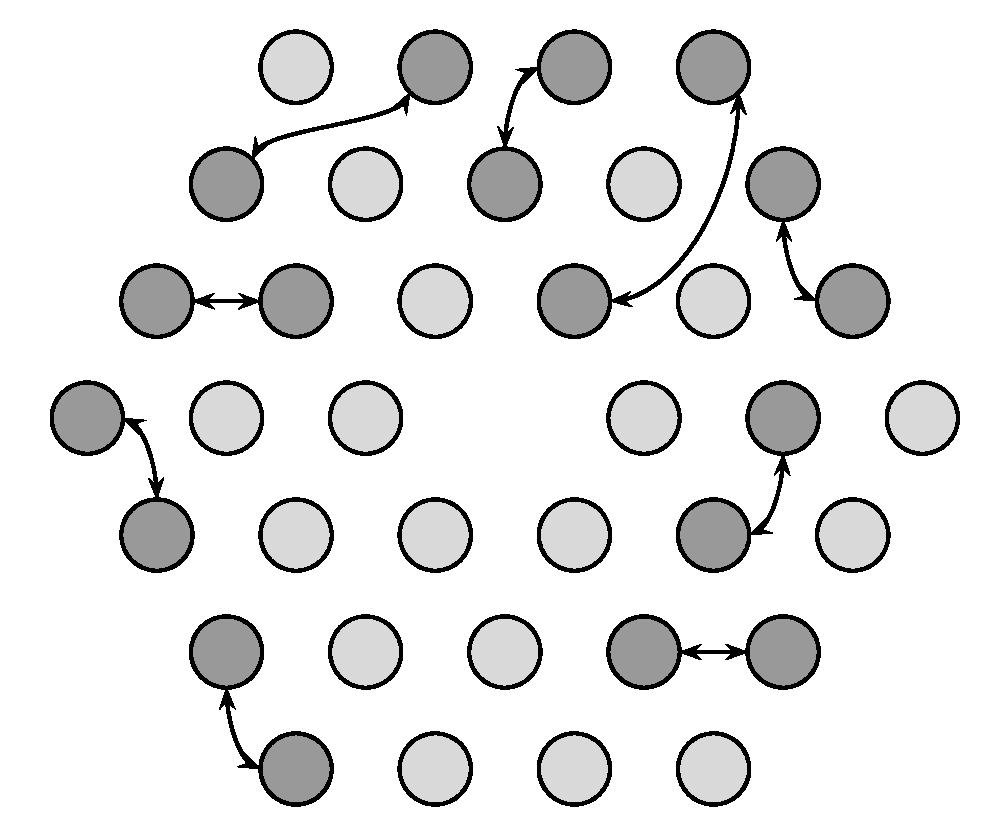
\includegraphics[width=0.4\textwidth]{ea}
			\caption{Example of an EA population, where some (dark grey) have fitness scores rewarding them with reproduction.}
			\label{fig:ea}
		\end{figure}
		
		Some schemes for parallelizing EAs are mentioned by \cite{sudholt15}. Among those mentioned are the master-slave model,
		Independent runs, Island models, and cellular EAs. In the master-slave model expensive operations are distributed to
		slaves and are synchronized from a master processor. With independent runs multiple serial EA's are run in parallel to
		increase the probability of finding an optimal solution. Independent runs do however have the drawback of some runs
		getting stuck with poor solutions, and the island model attempts to handle this by communicating the current best
		candidates between the EAs.
		
		The scheme can also be thought of as a single large population with subgroups that have limited communication. This
		idea is also reflected in nature, where members of a species separated by geography have more DNA in common with those
		from the same location than with others. Interestingly, this model is also well fit for application on GPUs, having a
		similar structure; individuals can be represented by threads, and islands by blocks. A GPU implementation of the
		island model can be found in \cite{luong10}, which examines various combinations of CPU and GPU computing. Running
		each island in a block keeps most	communication between threads in the same block which enables the use of fast shared
		memory, and limits the use of expensive inter-block communication that requires using slow global memory.
		\cite{luong10} notes however, that this limits the size of the population for each island and, by extension, in the
		whole system.
		
		\begin{figure}[h]
			\centering
			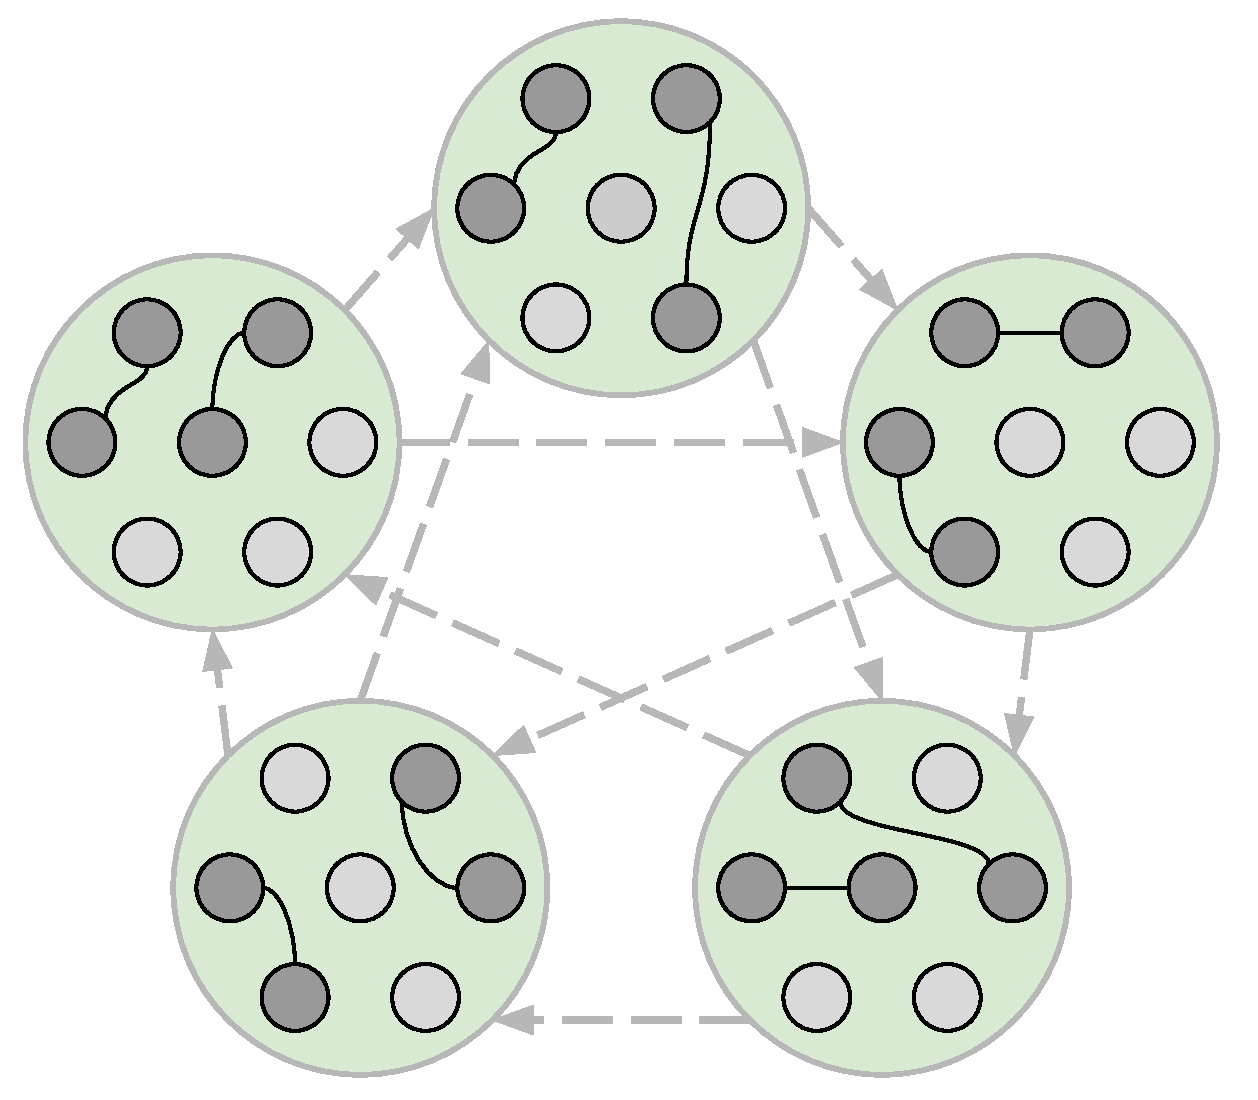
\includegraphics[width=0.4\textwidth]{island}
			\caption{With the island model, individuals on an island reproduce for some time, before migration occurs following some topology.}
			\label{fig:island}
		\end{figure}
		
		\cite{luong10} found the scheme to provide a significant speedup over a pure CPU implementation in their case, provided that the
		number of islands was large enough to cover global communication latency and that the population was small enough to
		fit in memory. While a naive implementation of EAs might perform poorly on GPUs the Island Model provides an easy fix, with great
		performance gains for a small implementation change. Luckily this change is great for GPU implementation, and does not
		impact the correctness of the algorithm, as EAs are heuristic.
		
%% Artificial Neural Networks %%
\section*{Scalable Massively Parallel Artificial Neural Networks}
	\subsection*{Problem}
		Artificial Neural Networks are another kind of heuristic solver for decision/behavior problems in AI, which is
		inspired by how the human brain works. Related to decision	trees, an ANN consists of multiple neurons, with weighted
		paths (synapses) between them. Given some input, values are propagated from the input nodes through layers of internal
		nodes in the network to some number of output nodes. Also like human brains, ANNs need to go through some learning
		process in order to recognize patterns and behave optimally.
		
		Given that ANNs operate propagating values from several nodes in a layer to nodes in the next, it is apparent that some
		parallelism may be exposed, but because of inter-node dependencies this may not be trivial. In addition to
		propagating values in parallel, learning may be parallelized by running multiple training sets at once and combining
		the resulting weights afterward.
	
	\subsection*{Algorithm}
		The ANN consists of a large number of nodes split into layers, at least one input and one output layer, as well as an
		unrestricted number of internal layers. A node on a layer is connected to some set of number on the preceding and
		succeeding layers. Each node takes as input the weighted values of its connected nodes from the previous layer,
		evaluates these inputs based on some function (often sigmoid of the sum), and outputs this value to all connected nodes
		on the next layer.
		\begin{figure}[h]
			\centering
			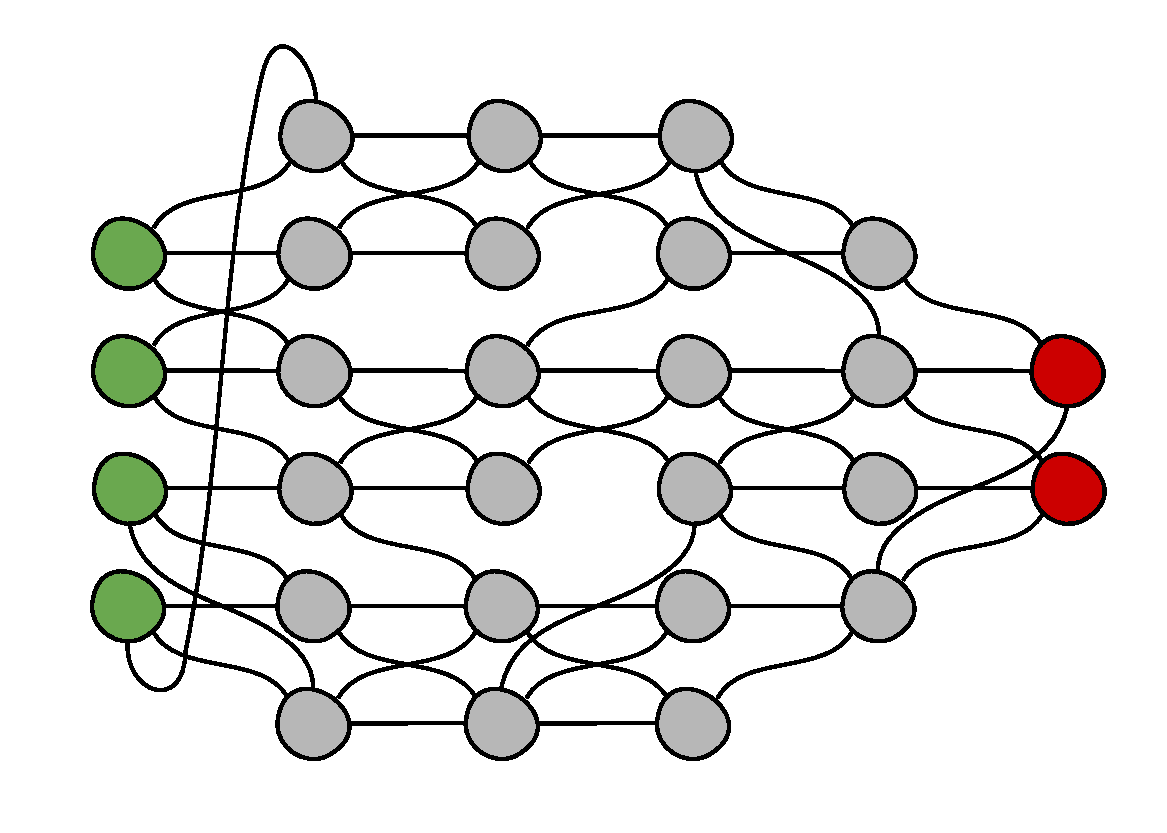
\includegraphics[width=0.4\textwidth]{ann}
			\caption{Example structure of an ANN, with input and output notes green and red respectively, and internal nodes in
			gray. Each connection will have some weight, and a node may have several incoming and outgoing connections.}
			\label{fig:ann}
		\end{figure}
		By running the training sets some configuration of weights is found that recognizes the correct
		output for any of the inputs. Assuming that the training sets are representative for the application, the ANN should
		now be able to correctly handle similar problems.
		
	\subsection*{Parallelization}
		Because of the possibly large number of dependencies between nodes (worst case is that every node on a level is
		connected to all nodes on the next), this is not trivial to parallelize. As mentioned one can run training sets in
		parallel, but we also want to parallelize for runtime. Using a similar scheme as for the EAs, one can partition
		the neurons/nodes into columns. A column may have a large number of internal connections, but few outgoing ones. This
		actually reflects the architecture of the brains neocortex to some degree, as it is divided into around half a million columns
		consisting of tens of thousands of neurons each.
		\begin{figure}[h]
			\centering
			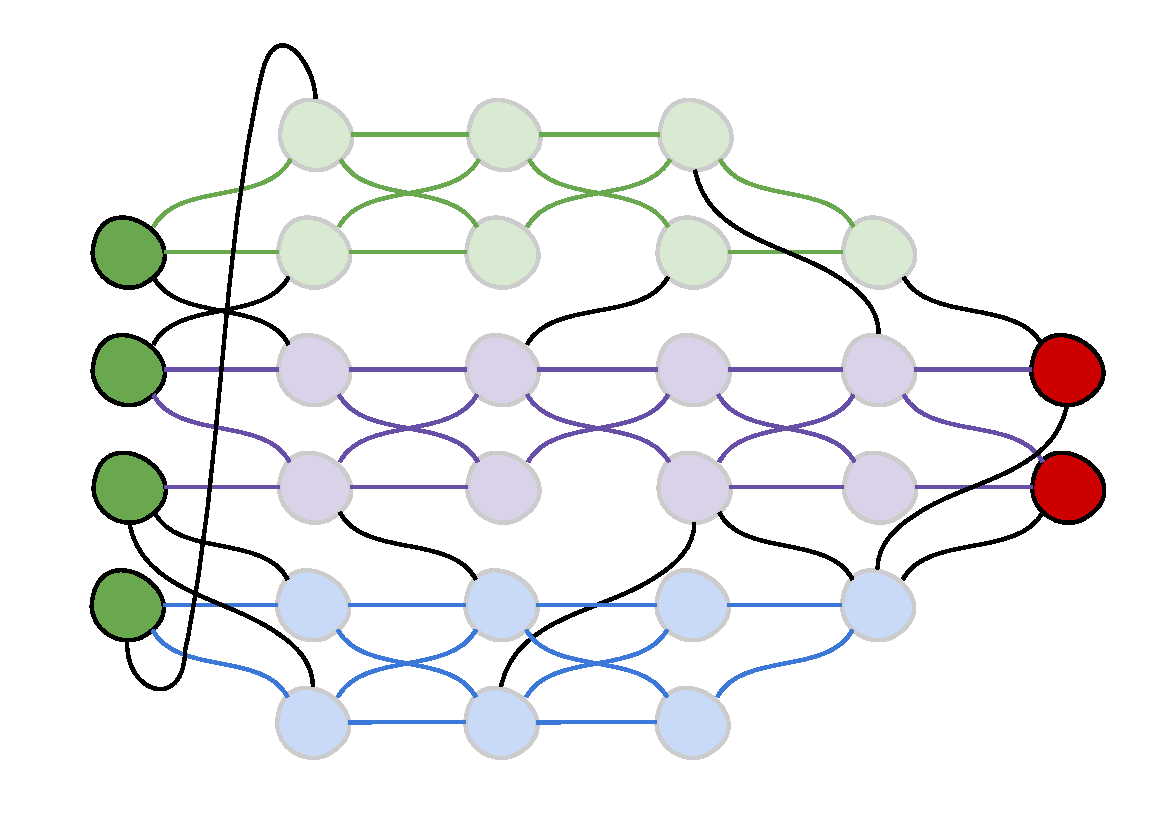
\includegraphics[width=0.4\textwidth]{cortex}
			\caption{Here the net is shown as divided into columns.}
			\label{fig:columns}
		\end{figure}
		
		The implementation described by \cite{long08} has extra neurons called ghost neurons acting as a border between columns,
		handling communication with other columns. Their result was a highly scalable and performant software, that actually
		reflects human brain physiology at least as well as a traditional ANN.
		
		While \cite{long08} successfully implemented the neural network for clusters, there are examples (\cite{jang08}, \cite{sierra10}) using
		GPUs either as accelerators for a system, or as part of the cluster. \cite{sierra10} used Nvidia's CUDA framework
		for GPGPU to accelerate training by implementing the backpropagation algorithm using a mix of cuBLAS and custom
		kernels. Using a single hidden layer, they report speedups of up to 63X over a CPU implementation. \cite{jang08} implements
		an ANN using both CUDA and OpenMP, splitting the workload to work around the bottleneck that is GPU memory.
		
%% Frequent Itemset Mining %%
\section*{Accelerating frequent itemset mining on graphics processing units}
	\subsection*{Problem}
		Frequent itemset mining (FIM) is a technique for finding frequently appearing subsets within a larger database of sets. What
		counts as frequent is defined by setting some threshold for minimum support. Examples of applications for this
		technique is web log mining or e-business, where the goal may be to detect which items are often bought together. \cite{zhang13}
		gives as definition of FIM "Given a transaction database and a minimum support, find all the item subsets with
		occurrence frequency higher than the given threshold."
	\subsection*{Algorithm}
		The naive method for finding the frequent itemsets would be to generate all possible sets, and log the frequency of
		each. It is readily apparent based on the exponential complexity alone that this is an undesirable approach.
		Great improvements over this have been made, both with regards to the generation of candidate sets and the counting
		step. Candidate generation has been done by joining smaller frequent subsets, knowing that no frequent itemsets have
		infrequent subsets, and Equivalent Class Clustering has reduced the cost of the join by preventing generation of
		redundant candidates. 
		
	\subsection*{Parallelization}
		\cite{zhang13} suggests the Frontier Expansion algorithm, which utilizes GPU acceleration and aims for a dynamic tradeoff
		between performance and memory. The algorithm is based on Equivalent Class Clustering (Eclat) method, and primary goal
		was to parallelize its computational kernel for GPUs. All candidates are stored in a "Frontier Stack" data structure
		CPU-side, which contains a reference to each candidates bit-set vertical transaction list.
		
		This frontier is then expanded by generating new candidates based an old one, consuming it in the process, and
		deleting infrequent itemsets. This is all done CPU-side, while the GPU handles the support counting, intersecting the
		vertical transactions lists. To improve performance \cite{zhang13} implemented a vertical list manager to handle frequent
		creation and deletion of lists, avoiding expensive memory allocation calls.
		
		\begin{algorithmic}
			\State $\text{Data preprocessing}$
			\While{$\text{not done}$}
				\State $\text{Candidate generation}$\Comment{CPU}
				\State $\text{Support counting}$\Comment{GPU}
				\State $\text{Removal of infrequent items}$\Comment{CPU}
			\EndWhile
		\end{algorithmic}
		
		The preprocessing step consists of converting all transactions to a vertical format, removing infrequent items that
		cannot appear in any frequent item set, and sorting items by frequency. Transactions are originally horizontal, stored
		as transactions with items, but are converted to a vertical format where each row contains an item along with a
		bitvector denoting transaction membership.
		
		\cite{zhang13} makes use of Equivalent Classes (EC), where two candidate sets are of EC if they have the same size $k$,
		and share a $k-1$ prefix, such that the $k-1$ items in each set are the same. The frontier stack is grouped by EC, and
		expansion is done by popping elements from the top and self-joining them to create a new candidate. These are then
		counted GPU-side, and if of sufficient frequency they are pushed to the stack. Keeping the list sorted with respect to
		EC, new candidates are generated until the list size is equal to the number of blocks that can run on the GPU.
		
		Support counting is done running a bitwise $and$ to intersect the two lists, with threads in a block operating on a
		word-length subset of the same list. \cite{zhang13} outlines how they support using multiple GPUs using a producer consumer
		model. Each EC can be expanded separately, and after initialization the producer thread distributes the frontier set
		among consumer threads.
		
		On datasets that match the preferences of the algorithm, with respect to size and ratio of items to transactions, the
		algorithm is found to perform well. Compared to some of the other problems mentioned above however, FIM does not
		appear to be as easy to parallelize.
		
	\section*{Conclusion}
		Having looked at some instances of parallelization it is apparent that one will always face some issues, but in many
		of the cases above workarounds were found that either avoided speedup penalty by rethinking the distribution of work,
		or even changed the way the algorithm worked, without sacrificing either performance or correctness. While many
		algorithms can be accelerated by multithreading we can see that some fit better than others, without being
		embarrassingly parallel from the start.
		
	\begin{thebibliography}{5}
		\bibitem{elster94}
			A. Elster,
			\emph{Parallelization Issues and Particle-In-Cell Codes}.
			Cornell University,
			1994.
			
		\bibitem{bird13}
			R. Bird, S. PennyCook, S. Wright, S. Jarvis,
			\href{http://eprints.dcs.warwick.ac.uk/1753/1/bird-iwocl2013.pdf}{
			\emph{Towards a Portable and Future-proof Particle-in-Cell Plasma Physics Code}.}
			1st International Workshop on OpenCL,
			University of Warwick,
			2013.
			
		\bibitem{satish09}
			N. Satish, M. Harris, M. Garland,
			\emph{Designing Efficient Sorting Algorithms for Manycore GPUs}.
			Parallel Distributed Processing,
			2009.
			
		\bibitem{sudholt15}
			D. Sudholt,
			\emph{Handbook of Computational Intelligence, ch Parallel Evolutionary Algorithms},
			Springer,
			2015
		
		\bibitem{luong10}
			T. Luong, N. Melab, E. Talbi,
			\emph{GPU-based Island Model for Evolutionary Algorithms}.
			Genetic and Evolutionary Computation Conference,
			Portland,
			2010.
			
		\bibitem{long08}
			L. Long, A. Gupta,
			\emph{Scalable Massively Parallel Artificial Neural Networks}.
			Journal of Aerospace Computing, Information, and Communication,
			American Institute of Aeronautics and Astronautics, Inc.,
			2008.
			
		\bibitem{sierra10}
			X. Sierra-Canto, F. Madera-Ramirez, V. Uc-Cetina,
			\href{http://ieeexplore.ieee.org/xpls/abs_all.jsp?arnumber=5708849}{
			\emph{Parallel Training of a Back-Propagation Neural Network using CUDA}.}
			Ninth International Conference on Machine Learning and Applications,
			Universidad Techno\'ogica Metropolitana,
			2010.
			
		\bibitem{jang08}
			H. Jang, A.Park, K. Jung,
			\href{http://ieeexplore.ieee.org/xpls/abs_all.jsp?arnumber=4700015}{
			\emph{Neural Network Implementation Using CUDA and OpenMP}.}
			Digital Image Computing: Techniques and Applications,
			Soongsil University,
			2008.
			
		\bibitem{zhang13}
			F. Zhang, Y. Zhang, J. Bakos,
			\emph{Accelerating frequent itemset mining on graphics processing units}.
			The Journal of Supercomputing, Springer,
			2013.
						
	\end{thebibliography}
\end{document}
